
\index{itk::MultiResolutionPyramidImageFilter|textbf}


\begin{figure}
\center
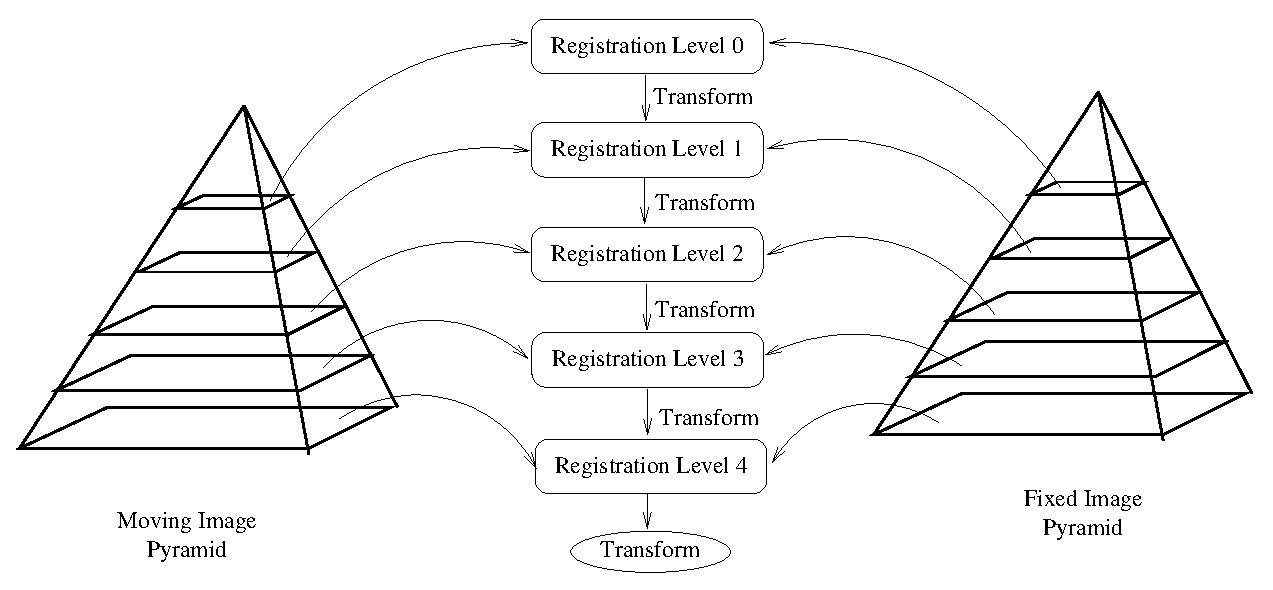
\includegraphics[width=14cm]{MultiResRegistrationConcept.eps}
\caption{Conceptual representation of Multi-Resolution registration.}
\label{fig:MultiResRegistrationConcept}
\end{figure}

Figure \ref{fig:MultiResRegistrationConcept} illustrates the high level concept
behind the multi-resolution registration framework implemented in ITK.



In ITK, the \code{MultiResolutionPyramidImageFilter} can be used to create a
sequence of downsampled version of the input image.  The downsampling is done
according to a user defined multi-resolution schedule. The schedule is
specified as an \code{Array<int>} containing shrink factors for each
multi-resolution level (rows) for each dimension (column).



